\section{List Mode Viewer}
This window is launched from within the main spectrum viewer application. Upon launching there are four individual graphs, seen in Figure \ref{fig:lmv}. This is used to split the list mode data acquired using the sync pulse and detector data. This will split that data relative to a sync pulse with an offset, with the data before the divider being referenced herein as region 1 and data after the divider as region 2.

\begin{figure}[h!]
	\centering
	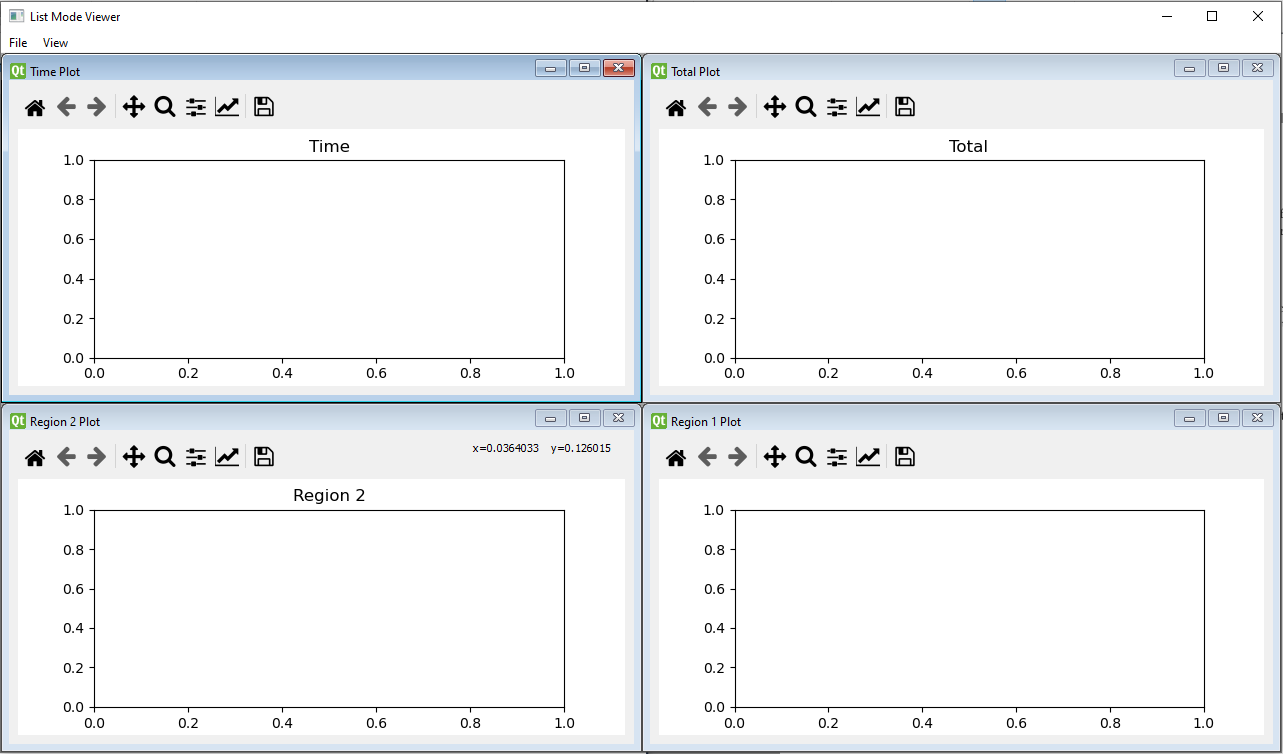
\includegraphics[width=\linewidth]{list_mode_viewer.png}
	\caption{Initial launching of list mode viewer}
	\label{fig:lmv}
\end{figure}

The top left graph will display the arrival of the pulse relative to the sync pulse. Top right will display the total spectrum as well as split data (region 1 \& 2). Bottom left will display only the region 2 spectrum, and the bottom right will display region 1 data.

\subsection{File Menu}
\subsubsection{Load New Data}
This launches the interface seen in Figure \ref{fig:new_loader}. The sync pulse and detector pulse are comma seperated files, corresponding to there respective files. It is expected that the comma seperated file will be in the form of having time, in nanoseconds, in the first column and a channel number being the second column. Once the files are loaded, the browse buttons with change to green. The final option is to add a calibration file, having been generated using the ``Calibrate Spectrum'' functionality. This is required to generate detection probability.
\begin{figure}[h!]
	\centering
	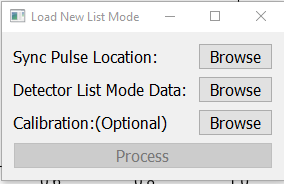
\includegraphics[width=0.5\linewidth]{load_new_viewer.png}
	\caption{List mode viewer data loader}
	\label{fig:new_loader}
\end{figure}
